\chapter{Introduction}
\pagenumbering{arabic}
\setcounter{page}{1}




Earth, our home planet, is the only known place in the universe that is affirmed to host life  \cite{daly2007introduction}. Our life on earth is characterized by three components, air, land, and water. Each element has its special property and is required in its proper proportions to maintain the healthy life of all living beings \cite{daly2007introduction}. %The quality of life relies on the quality of the environment. 
However, industrial development and other manmade activities create an imbalance in the natural environment. The process of making \iffalse land, water, air, and other parts of the \fi environment unsuitable and unsafe for the living condition by introducing substances that are harmful to the surroundings is called pollution \cite{manisalidis2020environmental}. Pollution changes the quality of the environment and is transboundary, as the pollutants travel thousands of mile \cite{daly2007introduction}. The presence of pollutants in the environment makes an adverse impact on human health and surrounding \cite{ritter1995persistent}. Many types of pollutants also contribute to global warming and climate change which are one of the major issues tackled by environmental scientists these days. Out of different types of pollution, human-influenced air pollution plays a major role in climate change as well as in international public health issues \cite{manisalidis2020environmental}.
 

 %are non-biodegradable and resist degradation by microorganisms; therefore they remain in the ecosystem causing adverse impact on human health and environment \cite{pops}. Global warming and related climate change are one major issues tackled by the environmental scientist.Environmental scientists these days mainly face problems related to global warming and climate change.
  

 Air pollution can be referred to as to the release of pollutants into the environment that is unfavorable to human wellbeing and the planet in general. According to the State of Global Air \cite{HealthEffectsInstitute2017}  the air pollution is a complex mixture of gases and particles whose sources and composition vary over space and time. 
  Air pollution over a region can be directly related to the development of industries, human activities, and other natural activities like volcanic eruptions, forest fires, etc. Contamination of air is a matter of serious concern and the public is often unaware of the impact that it causes to human health as well as to the surroundings. The World Health Organization (WHO) reported that the death rate estimates are around 7 million every year as 9 out of 10 people breathe polluted air \cite{Wolman1985}. This has led many motivated individuals like researchers and communities to work towards creating awareness among the people.
 
 There has been an enormous number of studies done to understand air pollution. Most of them involved in observing one or more pollutants of interest that are dominant in the area of measurement. Some other works focuses on improving the quality of the collected data, and also on effective visualization. With the development of sensor technologies, it is made possible to work more efficiently to understand air pollution. These sensors are low-cost, portable, and can measure specific air pollution. In our work, we have tried to create a complete system using low-cost sensors that measures a set of pollutants. The data collected from the system are calibrated and then visualized using a software tool. In this way, we have tried to simplify the complexity of building a complete system. 
 
 In the following section, we will discuss the background to introduce my research work and how air pollution is being currently measured in Prince George.
 
 
% The reason on choosing my research topic is that, I always wanted to work towards a social concern.
  %Various studies are underway on air pollution due to its increasing effect on the environment day by day.

 %This brings to the reason why I choose to work on sensor network for air pollution and also due to my background in electronics. In the following section, I will discuss the background to introduce my research work.


 \section{Background}

 The success of the Industrial Revolution and urbanization led to the development and growth of the economy, society, and large scale industries. This involved the use of more mechanization and the introduction of new technologies that led to the release of harmful pollutants into the environment. The introduction of a variety of pollutants into the environment created an imbalance in the ecosystem throughout the world \cite{manisalidis2020environmental}. The declining quality of air has changed from a local issue to an international public health issue. The use of coal as an energy source in industries, for example contributed to black smoke pollution in Europe and North America \cite{heidorn1978chronology}. Coal was not just used in industries but also in houses for heating in winter which made the pollution even worse \cite{Al2016}. The use of coal resulted in serious health impacts on residents in urban areas that increased the mortality rate during the 19\textsuperscript{th} century. 
%The developed industries across Europe and North America used coal as major source of energy that contributed to black smoke pollution \cite{heidorn1978chronology}. Coal was not just used in industries but also in houses for heating in winter which made the pollution even worse \cite{Al2016}. These emissions resulted in serious health impacts on residents in urban areas that increased the mortality rate during 19th century. 
 \par
 One such important event in the history of pollution is the great smog of London which killed as many as 12,000 people, mostly infants. This was caused due to the combination of cold weather with smoke and lasted for several days \cite{wilkins1954air}. There was a string of similar events reported in New York, England, and other parts of the world around the same time. With several incidents contributing to the global pollution led to the development of various private and government entities for ensuring air quality. 
 %environment monitoring stations that measures a set of pollutants specific to their region. 
 
 Governments along with these environmental agencies established legislation like the Clean Air Act \cite{caa}, the Motor-vehicle Air Pollution Act \cite{portney1990air}, Air Pollution Control Acts \cite{apc} for a better quality of air. Apart from that, they took the initiative to monitor air pollution by installing systems that could measure the concentration of pollutants that is specific to the area of measurement and could give warnings to the public as well as industries regarding how polluted the atmosphere is.
 
 
 \subsection{Existing Environmental Monitoring Station}
 
 Government and environmental agencies are making an effort to install monitoring stations for understanding air quality. These agencies monitor the 'criteria' pollutants (also called as common pollutants) along with any special pollutant that is dominant in that area. These monitoring stations are fixed in a location and are operated by environmental agencies. The stations are equipped with instruments that not only monitor criteria pollutants but also analyze other parameters like wind speed, humidity, precipitation. These analytical instruments work by the principle of sampling of the air collected from the atmosphere.
 There are two main methods for pollutant sampling: passive sampling, and active sampling \cite{Balakrishnan2015}. These sampling techniques are considered as one of the most significant developments for air quality measurement and used widely for monitoring purposes. 
 
 \par
 
 In passive sampling, the pollutants are collected by a physical process such as diffusion through a static air layer or membrane. These pollutants in the air are adsorbed on the sampling media due to the chemical composition of the pollutants. The analysis of the pollutant on the sampling media gives the time-averaged contaminant concentration. %\cite{Environment2009}. 
 
 On the other hand, active sampling works with an air sampling pump which actively pulls the air through a collection device like a filter, and weighted concentration is calculated. However, these instruments have a major drawback of temporal resolution as they are large and need regular maintenance. These instruments are expensive and are financially impractical to expand to multiple stations. As an example table \ref{table:cost}, gives the average estimated cost for purchasing air quality monitoring equipment produced by the US Environment Protection Agency (EPA). The FTIR in table \ref{table:cost} is the Fourier Transform Infrared spectroscopy measures multiple gases. It can be seen that cost of individual instruments for measuring the pollutants is considerable. 

 \hspace{1 cm}
 
 \begin{table}[h]
   
   
     \begin{tabularx}{\columnwidth}{X|X}
         \hline
         Pollutant/Parameter           & Estimated cost    \\
         \hline
     
       $NOx$   & 10,4440         USD \\ 
       $SO_2$   & 35,000          USD \\ 
       $COx$   & 28,000          USD\\ 
       $Ox$   & 6,600            USD\\ 
       $PM$   & 37,700           USD\\ 
      
       FTIR Analyzer   & 100,000 USD\\ \hline
      
         
       
   \end{tabularx}
  % *FTIR: Fourier Transform Infrared spectroscopy measures multiple gases 
     \caption{Estimated cost of air quality monitoring equipment obtained from EPA air pollution control cost manual published for the year 2000 \cite{Mussatti2000}}
     \label{table:cost}
   \end{table}
 
 
   \hspace{1 cm}

 As a result of the high cost, only a few monitoring stations are installed for an area. We can claim that spatial resolution is limited to these conventional monitoring systems. This has led researchers and scientists to work on portable and less expensive sensor networks to understand air pollution in more detail.
 


 
\section{Air Pollutants and Measurement Metrics}


Various pollutants contribute to the contamination of the environment. These pollutants differ from region to region depending on human activities. For example, in an industrial area that manufactures products from raw materials, such as the production of iron from its ore or production of gasoline from crude oil, releases inorganic carbon compounds into the atmosphere \cite{Vallero2014}. These pollutants released from industrial activities can have a huge impact on human health as well as the ecosystem.  %Urban areas are major sources of particulate matter and carbon compounds produced from the burning of fuels in vehicles.



One of the pollutants of most serious health concerns is Particulate Matter. Particulate matter is described as the particles that are formed in the atmosphere due to a chemical reaction between different pollutants in the environment \cite{manisalidis2020environmental}. These particles vary in their diameter and are measured at two levels; fine particles which are 2.5 microns or less in size ($PM_{2.5}$) and coarse particles which are 10 microns or less in size ($PM_{10}$). These are measured in terms of concentration in micrograms per cubic meter ($\mu g/m^3$) \cite{Wilson1997}. The fine particles are formed by foamed aerosols, metal vapors, and combustion particles. The coarse particles are formed from the break up of larger particles and contain road dust, earth crust materials, and industrial particles. 



The generation of both fine and coarse particles is from industrial activities, factories, construction, burning of fossil fuels, or even vacuuming. The varied composition of size can be related to the source where the particle is generated. The figure \ref{PMSIZE} shows the range of size that particulate matter can vary on a logarithmic scale along with the range of other components  \cite{world2006air}. The $PM_{10}$, $PM_{2.5}$ along with ultrafine particles shown in figure \ref{PMSIZE} are the particles that cause health issues like asthma, lung disease, heart attacks, and other serious issues like cardiovascular and respiratory diseases. They are capable of penetrating through the lungs leading to cardiovascular and Chronic Obstructive Pulmonary Diseases (COPD) \cite{Tian2016}. 





\hspace{1 cm}

\begin{figure}[h!]
  \begin{center}
  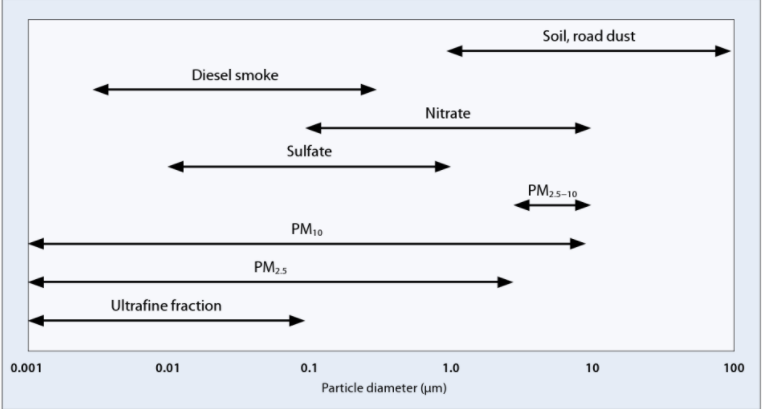
\includegraphics[scale=0.93]{./images/figure37.png}
  \end{center}
 
  \caption{The size of Particulate Matter including $PM_{10}$, $PM_{2.5}$ and ultrafine particle \cite{world2006air}}
  
  \label{PMSIZE}
\end{figure}
\hspace{1 cm}

\par
The next pollutant on the list is Carbon Monoxide ($CO$) that is produced from incomplete combustion of fossil fuels such as motor vehicle emission \cite{Payus2019}. The majority of the $CO$ present in the atmosphere is from road traffic and the rest is from the burning of other fuels \cite{Payus2019}. Exposure to $CO$  which is a colorless and odorless gas, results in absorption of the gas into the bloodstream and reduces the ability of lungs to transfer oxygen which in turn affects the functionality of vital organs such as the brain and the heart \cite{Sierra-vargas2012} \cite{Golbabaei2012}.

Another vehicle emitted gas that harms air quality is Nitrogen Dioxide ($NO_2$). Nitrogen is the most abundant element in earth's atmosphere and is approximately 78\% by volume \cite{EnvironmentalQualitySectionMoE2012}. There are five forms of gaseous Nitrogen: Nitrogen (${N_2}$), Nitrogen Dioxide ($NO_2$), ammonia ($NH_3$), Nitrous Oxide ($N_2O$), and Nitric Oxide ($NO$). The combustion of motor vehicle exhaust, industrial process, fuel combustion for heating produces $NO$ which is easily oxidized to $NO_2$ \cite{EnvironmentalQualitySectionMoE2012}. $NO_2$ can cause adverse pulmonary disease when inhaled in high concentrations and causes illness such as wheezing, coughing, bronchitis, and increases the severity of flu symptoms\cite{Salonen2019}. 

The next serious pollutant present is Ground Level Ozone ($O_3$) which is formed from a chemical reaction between pollutants like oxides of Nitrogen and Volatile Organic Compounds (VOCs) with sunlight \cite{EPA2018}. Ozone can also be produced when there is a reaction between oxides of Nitrogen and hydrocarbons in the presence of sunlight \cite{Environment2016}.  The rate of production of Ozone increases at high temperature and in the presence of sunlight. Respiratory issues such as a decrease in responsiveness of airways, inflammation in airways, breathing difficulties and lung infectivity occur due to exposure of high concentration of ozone ($O_3$) \cite{Lippmann1989}. Ozone can also decrease the productivity of vegetation and crops \cite{cukor2015bridging}. These are the most common pollutants seen almost everywhere but there are also other pollutants like Lead ($Pb$) or Benzene ($C_{6}H_{6}$) depending on the industrial activity in that area. All these pollutants can cause severe health impacts and also reduce life expectancy or even could cause death.

Based on the severity of health impact and the kind of human activities, different government agencies around the globe have taken measures to preserve the environment. Each country developed its indexes to identify the impact of pollution on the surroundings. For this, they might include a specific set of pollutants that are local to the region and varies from region to region.For example, in the United States, the Environmental Protection Agency (EPA) established the National Ambient Air Quality Standards (NAAQS) that specifies the pollutants that are harmful to the public health and environment. The NAAQS has a set of six common criteria pollutants that harm human health, the environment, or even cause property damage. The pollutants specified by NAAQS are Particulate Matter ($PM$), Ozone ($O_3$),  Nitrogen Dioxide ($NO_2$), Carbon Monoxide ($CO$), Sulphur Dioxide ($SO_2$), and Lead ($Pb$).

India on the other hand measures eight major pollutants; Particulate matter ($PM$), Ozone ($O_3$), Nitrogen Dioxide ($NO_2$), Carbon Monoxide ($CO$), Sulphur Dioxide ($SO_2$), Ammonia ($NH_3$), and Benzene ($C_6H_6$) (in some places ($Pb$) instead). Most other countries measures a subset of these criteria pollutants, for example, Canada measures $PM$, $O_3$, $NO_2$, $SO_2$ and $CO$ \cite{Chen2013}. Each country has identified a set of pollutants and measurement units for these pollutants. %The most popular units used to measure these pollutants are either in parts per million ($ppm$) or in parts per billion ($ppb$). 
For a laymen to understand these individual measurements and its cumulative impact on the quality of air is challenging. 
%These individual measurements are not provided in laymen terms and therefore are not helpful in understanding the cumulative impact of the air quality. 
Taking this into account, the government agencies of each country has developed their indices similar to the NAAQS for representing the quality of air. A wide range of indices have been proposed like Air Quality Health Index (AQHI), Air Quality Index (AQI), Air Pollution Index (API), Pollution Standard Index (PSI), Comprehensive Air Quality Index (CAI), Daily Air Quality Index, Common Air Quality Index (CAQI) are few used in different countries \cite{WinNT}. Out of all these indexes, the most common is AQI and AQHI which are proposed and used by different countries \cite{Chen2013}.

India, USA, UK, and many other countries use AQI, and Canada, Hong Kong uses AQHI. These metrics are designed by carefully examining those pollutants which are harmful to human health and the environment.
The AQI is defined as a piecewise linear function of the pollutant concentration \cite{Soni2016} and is measured using the following formula.

\begin{equation}
AQI = Max \{I_i|i = 1, ..., 8\}
\end{equation}
where $I_i$ is an air quality sub-index corresponding each pollutant and it is computed as 
\begin{equation}
I_i = \lceil(\frac{I_{high} - I_{low}}{C_{high} - C_{low}})\rceil \times (C - C_{low}) + I_{low}
\end{equation}
where $C$ is concentration of the $i^{th}$ pollutant. $C_{low}$ and $C_{high}$ are lower and upper concentration breakpoints of $C$ respectively.
$I_{low}$ and $I_{high}$, respectively, are index breakpoints corresponds to $C_{low}$ and $C_{high}$.  The value of AQI varies from 0 to 400+ as shown in Figure \ref{aqi} and is color-coded to show the quality of air in the atmosphere. This index is described to the public by categorizing into six categories: good (0-50), satisfactory (51-100), moderately polluted (101-200), poor (201-300), very poor (301-400), and severe (>401).


\begin{figure}[h]
    \begin{center}
    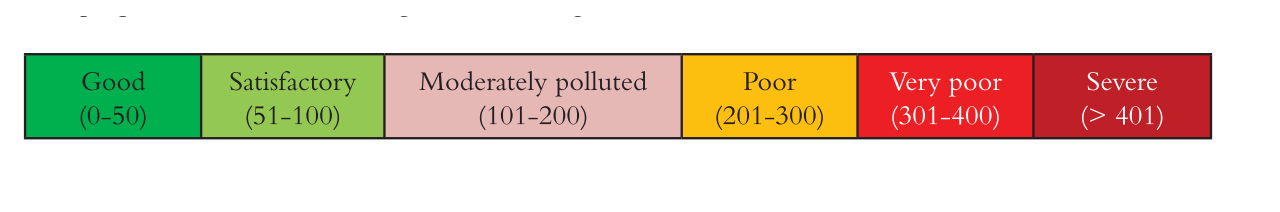
\includegraphics[scale=0.58]{./images/figure13.png}
    \end{center}
   
    \caption{The numerical scale of Air Quality Index (AQI) showing the six categories \cite{AirQualityIndex}}
    
    \label{aqi}
\end{figure}

\hspace{1 cm}

In past Canada used the USA's AQI for understanding the air quality. Due to some concerns raised by provincial and municipal health authorities, Health Canada along with Environment and Climate Change Canada (ECCC) developed AQHI to make the public aware of the quality of air that surrounds them and how it affects their health. The basis of generating this newer metrics is to understand how air quality affects human health and this is achieved by statistically linking the pollutant data with the outcomes of human mortality \cite{hasselback2010air}. Initially, it was based on five major pollutants $PM_{2.5}$, $O_3$, $NO_2$, $SO_2,$ and $CO$ initially and later the last two pollutants were dropped from the calculation as they were identified to contribute less in predicting health effects. The following formula computes AQHI.
%look into equation and see what is it? ppm or ppb?





\begin{equation}
AQHI = \lceil (\frac{1000}{10.4}) \times [e^A-1]+[e^B-1]+[e^C-1] \rceil
\end{equation}

where $ A = 0.000537 \times$ concentration of  $O_3$ ($ppb$), $B = 0.000871 \times$ concentration  of $NO_2$ ($ppb$) and  $C = 0.000487 \times$ concentration of $PM_{2.5}$ ($ug/m^3$).


\begin{figure}[h!]
  \begin{center}
  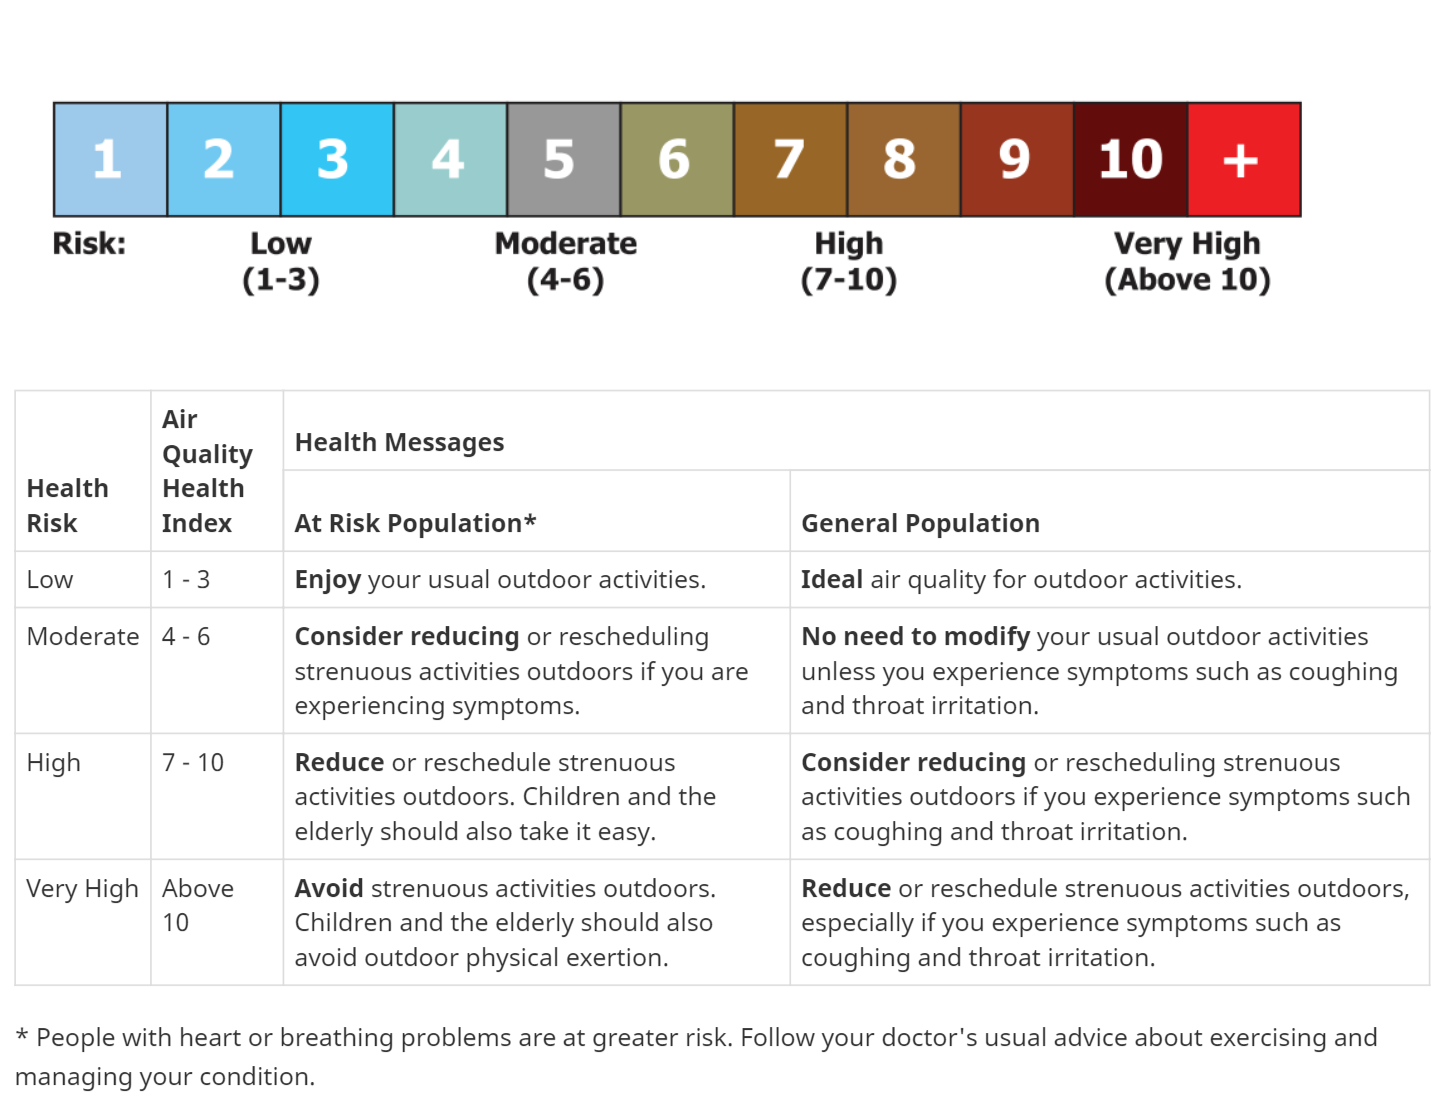
\includegraphics[scale=0.25]{./images/figure103.png}
  \end{center}
 
  \caption{The numerical scale of Air Quality Health Index (AQHI) and the health message table given by ECCC associated to each of the categories \cite{healthmess}} 
  
  \label{aqhi}
\end{figure}
\hspace{1 cm}





The value of AQHI can belong to any one of the four health risk categories as shown in figure \ref{aqhi}. AQHI value from 1 to 3 - low health risk, value between 4 to 6 - moderate health risk, AQHI value from 7 to 10 - high health risk, and value above 10 - very high health risk. There are also health messages associated to each category for alerting the public about the potential health effects when exposed to poor air quality shown in Figure \ref{aqhi}. The value of AQHI gives the risk level based on the exposure to pollution level as people get affected when they are exposed to pollution. In this way by identifying the value of AQHI the people can avoid the short-term exposure to pollution and help to build community with better air quality.  

 %The AQHI was created with a different objective in mind, which is to provide information on the effect of pollutants on human health. AQI is based on a single dominant pollutant and hence it is harder to see its direct relationship with health \cite{Chen2013}.%which gives more close relation to the mixture of air pollutant than AQI. It is to be noted that both the indices failed to project the health outcomes associated with the exposure to the polluted environment \cite{Chen2013}. 



%\section{Impact of Air Pollution}

%Air pollution has significantly increased as a result of industrialization and urbanization. The burning of fossil fuels, exhaust from factories and industries, and mining operations are major contributors to air pollution. Exposure to air pollutants causes premature deaths, cardiovascular disease, stroke, and other respiratory diseases. The State of Global Air 2017 report \cite{HealthEffectsInstitute2017} has discussed the effects of long-term exposure to harmful air pollutants such as particulate matter which contributes to over 4 million premature deaths and is estimated to double by 2050 if the issue remains unattended. Air pollution accounts for the highest death rates annually. 

\par





 \section{Air Quality measurement in British Columbia (BC)}

 Air quality monitoring in BC is measured by the provincial government, Metro Vancouver along with Environment Canada and regional districts. There are around 150 stations for air quality measurement and these are maintained by Ministry of Environment (MOE) and some industrial employees with permit \cite{bc}. The main pollutants of interest in BC are Carbon Monoxide ($CO$), Nitrogen Dioxide ($NO_{2}$), Ozone ($O_{3}$), Particulate Matter ($PM_{2.5}$ and $PM_{10}$), Sulphur Dioxide ($SO_{2}$), and Hydrogen Sulphide ($H_{2}S$). These pollutants are measured in three ways: continuous monitoring, non-continuous monitoring, and mobile monitoring \cite{bc}.
 
 \begin{enumerate}


  \item Continuous monitoring: This is an automated mode of measurement in which air quality is measured by drawing air through tubes. The collected air is automatically monitored, measured, documented, analyzed and validated. This data is then further checked for any errors and made available to public in an hourly manner in the current air quality data page by MOE.
  
\begin{comment}
  

  
 \begin{table}[h]
   
   
  \begin{tabularx}{\columnwidth}{X|X}
      \hline
      Instrument name         & Pollutant/Parameter measured   \\
      \hline
     \\
     Tempered Element Oscillating Microbalance (TEOM)  &     Particulate Matter ($PM_{2.5}$ and $PM_{10}$)     \\ 
     Beta Attenuated Monitoring (BAM)                  &     Particulate Matter ($PM_{2.5}$)                   \\ 
     UV Photometry                                     &     Ozone ($O_{3}$)                                   \\ 
     Chemiluminscence                                  &     Nitrogen Dioxide ($NO_{2}$)                        \\ 
     UV Fluorescence                                   &     Sulphur Dioxide ($SO_{2}$)                         \\ 
     Pulsed Fluorescence                               &    Total Reduced Sulphur (TRS) or Hydrogen Sulphide ($H_{2}S$) \\
     Nondispersive Infrared Photometry & Carbon Monoxide($CO$)\\ 
     
     \\
     
     \hline
   
  
    
\end{tabularx}
% *FTIR: Fourier Transform Infrared spectroscopy measures multiple gases 
  \caption{Instrument used and parameters measured in BC province}
  \label{contmont}
\end{table}
  
\end{comment}

  \item Non-continuous monitoring: The non-continuous monitoring is also called as manual sampling. In this method the field technicians assigned by the ministry collects the air sample by placing filters or canisters for a discrete period of time (such as one, three, or six days). The sampling follows strict rules set out by the MOE. The collected sample is then sent to the certified labs where it is weighed and examined to understand the content and then the information is uploaded to the database of MOE. The manual instruments used to collect the sample values are Single Channel 16.7l/m (PM2.5 and PM10) monitors, Dichotomous (Coarse and Fine PM) monitors, Speciation monitors, VOC monitors, PAH monitors, and Passive samplers.
  


  \item Mobile monitoring: The last method for collecting the data is by installing monitoring instruments in a large vehicle or an airplane. These instruments move around for short period collecting data around areas where fixed monitoring is not available. One such air quality monitor is  Mobile Air Monitoring Laboratory (MAML) \cite{MAML} build on Ford F550 chassis which can measure both continuous and non-continuous measurement. 
  
  \vspace{5mm}


  \begin{figure}[h]
    \begin{center}
    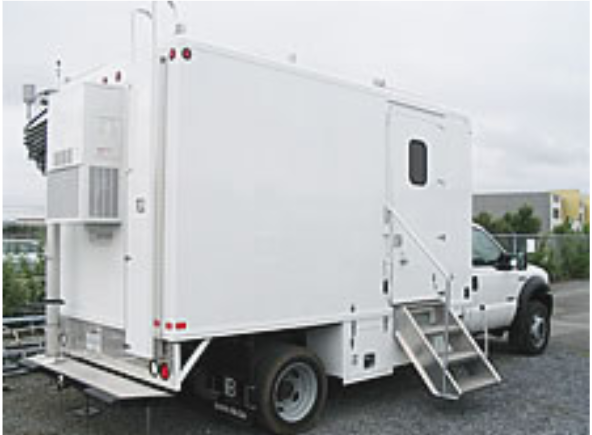
\includegraphics[scale= 0.65]{./images/figure38.png}
    \end{center}
   
    \caption{ The Mobile Air Monitoring Laboratory Vehicle in BC \cite{MAML}}
    
    
    \label{MAML}
   \end{figure}

   \vspace{5mm}



  



The common air pollutants measure by MAML are black carbon, Sulphur Dioxide, Nitrogen Dioxide, Carbon Monoxide, Ozone, and Particulate Matter (PM). 
It also measures meteorological data like wind speed, wind direction, temperature, and humidity.
The collected data is then analyzed and transferred to the database of the ministry.

\end{enumerate}



 \subsection{Pollution Monitoring System in Prince George}
 

 The city of Prince George is located in the central part of the BC province at the junction between the Nechako and Fraser rivers. The city has reported poor air quality due to forest fires, road dust, geographical location, transportation, industries, and other factors.
The air quality of an area can be directly related to human activities within the physical environment \cite{manisalidis2020environmental}.
 For this reason, it can be seen that there is a huge variation in the distribution of pollutants from region to region. For example; the presence of an industrial source such as a pulp mill in and around this area can highly affect the quality of air. Other factors include topography, atmospheric condition, and magnitude of emission from sources \cite{Prevention2000}. 
 
  

 Having considered all these factors over the years in Prince George, Government agencies along with industrial partners funded the installation of eight fixed monitoring stations to measure the dominant pollutants in the area \cite{Authority2011}. Figure \ref{Map} shows the layout of the eight monitoring stations located in the region as reported in the air quality report of 2016 \cite{Environment2016}. The data collected from these stations are monitored by the Prince George Air Improvement Roundtable (PGAIR)  which includes the Ministry of Environment (MOE), the Ambient Air Quality Monitoring Working Group, and other volunteers.
 




 \begin{figure}[h!]
  \begin{center}
  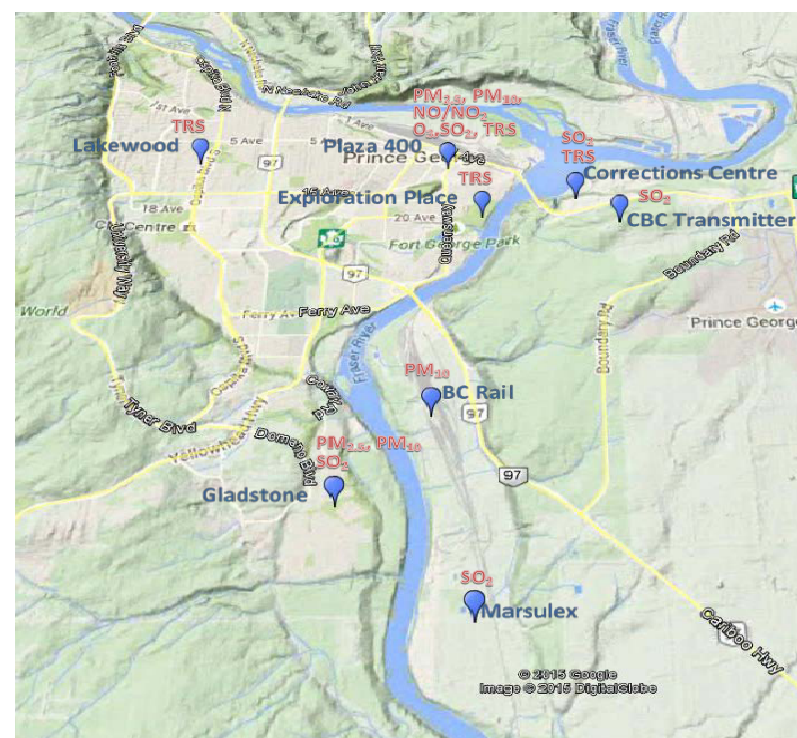
\includegraphics[scale=0.59]{./images/figure19.png}
  \end{center}
 
  \caption{Map showing the location of the eight monitoring station in Prince George \cite{Environment2016}}
  
  \label{Map}
  \end{figure}
 
  \vspace{5mm}
  




 Of the eight monitoring stations installed, there is a core station that measures all six pollutants which includes Particulate Matter ($PM_{2.5}$ and $PM_{10}$), Total Reduced Sulphur ($TRS$), Sulphur $SO_{2}$, $NO_2$, and ${O_3}$. The other stations only measure certain pollutants or meteorological data \cite{Environment2016}. The core station which is called the Plaza 400 monitoring station is located downtown and here the air quality can be recognized as a combination of industrial, commercial, and residential emissions \cite{Authority2011}. This station contains several instruments such as  API model 400 ozone monitor for ozone, API $NO_{x}$ monitor for Nitrogen Dioxide, SHARP model 5030 for $PM_{2.5}$), TEOM series 1400a analyzers for $PM_{2.5}$ and $PM_{2.5}$, and TRS samplers for Total Reduced Sulphur \cite{Environment2016}\cite{Authority2011}. These data are available in the MOE \cite{ MOE2020} website and the data can be accessed and downloaded by the public. The collected pollutant values are used to calculate the AQHI value which gives information about the local air quality that can help in determining health effects. %This can be seen in figure \ref{distribution} that shows the frequency of occurrence of indexes and the related health issues in town. It can be seen that between the year 2000 to 2006 the AQHI value varied mostly between 0 to 6 which is from low health risk to moderate health risk. During that time high AQHI value is very rare and can be accounted to less than 1\% of time \cite{hasselback2010air}.
 


\section{Motivation}

One of the important components in dealing with the issue of air pollution is to increase awareness among the public about the seriousness of air pollution that they can act. The conventional method of monitoring air quality with the help of a few expensive and stationary monitoring systems typically installed by government agencies may not be effective. To achieve the goal of public engagement, pollution monitoring must become part of daily activity for everyone. For that, the devices to monitor pollution must be small, portable, inexpensive, and part of a regional, national, and global system. With the technological advancement of low-cost computing, communication, and sensing devices, and the revolution of open source software \cite{Anthes2016}, we believe it is possible to build a pervasive air pollution monitoring system with the available sensors from the market and open-source software. Now the question is how to design such pollution monitoring systems faster and make them accessible to as many people as possible. 

\par

Achieving the above-stated goal requires a suitable system framework that can help to accelerate the process of the design and implementation of an air pollution monitoring system using the off-the-shelf hardware and building open source tools for representing the data collected from the sensors. This thesis is an attempt to build a simple and comprehensive system using low-cost sensors and demonstrating the value using a software tool. We have also added a step of calibration by implementing a web-based tool to ensure that we measure high-quality data. Our contribution is a step towards inspiring and motivating not only the public to use the device but also enable many amateur electronic hobbyists to buy and construct the hardware and download the associated software to build their pollution monitoring device.

\begin{comment}
\section{Research Problem}

This thesis focuses on design and development of an air pollution monitoring system using off-the-shelf
hardware and build an open source software that focuses on three different types of users with the following objectives in mind:
\begin{enumerate}
  \item To demonstrate the quality of data obtained from the low cost system by comparing it with the expensive monitors fixed at a particular location.
  
  \item To encourage citizen to contribute in solving the issue of air pollution and to give more insight about the impact it causes to human health and environment.
   
  \item To give an idea on how to integrate the hardware components to a processor and also make an independent software, which can be accessed world-wide.
  
  \item To provide user oriented data which gives a deeper understanding about the pollution.
  
  \item To provide information on the quality of air by including Air Quality Health Index (AQHI) which provides a measure of adverse affects on health by pollutants and Air Quality Index (AQI) that gives an idea about the level of pollution on the environment.

  
  \item Improving the quality of data obtained from the system by integrating a calibration tool.
  

   

\end{enumerate}


\subsection{Portable Sensor Network and Air Quality Monitoring}
 
 %FILL THE GAP BETWEEN THE FIRST AND SECOND SENTENCE.There is an emerging trend of using low-cost air sensors to understand the quality of air because of its low cost, small size and low power consumption \cite{Sun2016}.
 The development of Wireless Sensor Networks (WSN) has gained attention in various fields like military monitoring purpose, surveillance and tracking, traffic density calculation, road condition, and environmental applications \cite{Kadri2013}. Out of the many application for which sensor networks are used, measuring air pollution has gained a lot of attention. The mobility and feasibility of these sensor networks help individuals to understand the distribution of pollution in the surroundings. These sensors are cheaper than reference station equipment and can be replaced easily in case of damage. The advancement in Micro-Electro-Mechanical Systems (MEMS) has made it possible to integrate all the functions into a single electronic circuit which makes it more compact. These sensors do not incur substantial deployment cost, infrastructure cost, and does not require frequent maintenance, which makes the overall expense even less.
 \par
 
  Sensor units are portable and can be attached to an automobile, or placed on top of buildings, and even could be in a wearable form to track or understand the personalized effect of pollution. Sensors measuring different pollutants can be integrated to make a sensor node system. Using such a sensor node help to give a peek to how air pollution looks in a region and can also help to understand the personal exposure. Extensive research and development work has been done with the available sensors in the market. 
  

\end{comment}
\section{Thesis Contribution}

There are three major contributions from the thesis:
\begin{enumerate}
  
    \item Air pollution monitoring system: The system itself which measures the pollutants from the atmosphere. This includes the sensors with the processor and the data transferring module. We believe that this could be a way to show that a low-cost system could be used for data collection.
    
    \item  Air pollution visualization software: The next major contribution is the software that could be used for data visualization. The main idea is to make the collected data user-accessible and hence we came up with the idea of building the complete tool from the scratch as the other available tools in the market are costly. 
    
    \item Calibration tool: Development of a web-based tool for sensor calibration to ensure the quality of data obtained from the sensor system.
    
    %Macro Analysis Tool (MAT) developed by Environmental Protection Agency (EPA)\cite{airsensorguidebook} which is an excel based tool was modified into a web-based tool which provides an access for any user to understand the quality of data obtained.
  
\end{enumerate}
\begin{comment}
  


\section{Research Question}
 
 Some important research questions to be addressed related to the issue of air quality are: 

 \begin{enumerate}
 
  \item What kind pollutants affect the human health most? How to measure them?
   
  \item  As the pollution is in the atmosphere, should it not be measured everywhere all the time? If so, what kind of infrastructure is needed to facilitate such a ubiquitous measurement?
  
 \item What all factors should be considered while selecting sensors for measurement of pollutants?
 
 \item Which processor to be used for processing the data collected from sensors?
 
 \item How should the hardware component i.e the sensors and the processor, should be packaged?
 
 \item What is the difference between different metrics which is used to show the effect of pollution?

\item How can the seriousness of pollution be made aware?

 \item How can the representation of Air quality metrics be done?
 
 \end{enumerate}
 
\section{Research Challenges}


The major challenges experienced on creating a complete system are:

\begin{enumerate}


\item The integration of different sensors with the processor.
\par
As each sensor has its own property, there can be issues when connecting all of them together in a single platform. Most of the sensors used for measurement are heat sensor and needs to be powered at least 12 hours before operating. There is a particular operating temperature range for each sensor  connected. As each of the sensor needs different environment for working, all the factors should be incorporated for a complete working environment.



\item Calibration of each sensors based on the data sheet.
\par
As I am selecting low cost sensors which comes with calibration with respect to the environment it was developed. The collected data changes for each environment and this should be taken care of. This can be a tough task as for each of the sensors it changes based on the slope of internal resistance and the internal voltage values given in data sheet. 


\item Packaging of hardware component.
\par
To make the whole system portable it should be packed carefully. For certain sensor like dust sensor, it should be exposed to the environment so as to estimate the particulate matter. This packing should be done in such a way that the it does not hinder with the observed value.

\item Development of the visualization software.
\par The development of user specific visualization tool from the scratch was most challenging as this was my first hands on experience in creating a tool which involved different methods of data display. Another task was to make the tool connect to the backend python code which does the data clensing and calibration which took a lot of preparation work.

\item Transferring the data to a platform or a database using the WiFi module.

\item Checking whether the collected data is accurate.


\end{enumerate}
\end{comment}

\section{Structure of the Thesis}

The rest of the thesis is organized as follows. Chapter 2 focuses on a review of related work for different methods of understanding and detecting pollution. This is divided into four main categories and work done in each category is explained further. Next, in Chapter 3 the design and implementation of a pollution monitoring system and the visualization tool are explained. To test the accuracy of collected data to the original data we have implemented a calibration tool by linear regression which is described in Chapter 4. In Chapter 5, we present an analysis of the results obtained from the system. Finally, in Chapter 6 the conclusions and directions for future work are discussed.